% ==============================================================================
% Summary and Research Directions
% ==============================================================================

\subsection{What This Chapter Has Established}

This chapter presented a unified structural interpretation of weak-sector
phenomenology within the thick-brane framework of Elastic Diffusive Cosmology.
The core achievements are:

\subsubsection{A Unified Pipeline}

All weak decays---from neutron $\beta$-decay to pion leptonic channels---pass
through the same three-stage pipeline:
\begin{enumerate}
  \item \textbf{Absorption}: Energy pumping from bulk or mode excitation
  \item \textbf{Dissipation}: Mode redistribution within the brane layer
  \item \textbf{Release}: Frozen projection onto 3D observables
\end{enumerate}

The differences between particles arise from their ontological category
(bulk-core, brane-dominant, edge mode, composite) and kinematic thresholds,
not from fundamentally different mechanisms.

\subsubsection{Mechanistic Interpretation of Channel Selection}

The projection operator $\mathcal{P}_{\text{frozen}}$ provides a mechanistic
language for decay selection rules:
\begin{itemize}[nosep]
  \item $\mathcal{P}_{\text{energy}}$: Kinematic thresholds and phase space
  \item $\mathcal{P}_{\text{mode}}$: Wavefunction overlap requirements
  \item $\mathcal{P}_{\text{chir}}$: Chirality selection from boundary conditions
\end{itemize}

This transforms ``why does this decay happen?'' into ``what projection gates
are open?''

\subsubsection{Ontological Classification}

Particles occupy distinct positions in the 5D geometry:
\begin{itemize}[nosep]
  \item \textbf{Bulk-core junctions}: Neutron, proton (hadronic sector)
  \item \textbf{Brane-dominant modes}: Electron, muon, tau (leptonic sector)
  \item \textbf{Edge modes}: Neutrinos (at bulk-brane interface)
  \item \textbf{Composites}: Pions (junction-pair configurations)
\end{itemize}

This classification is not merely taxonomic; it determines dynamical behavior.

\subsubsection{Explicit Falsifiability}

Each case study includes explicit falsifiability hooks. The framework is
empirically vulnerable: if observations contradict the structural predictions,
the framework fails.

\subsection{What Remains Open}

\subsubsection{Priority 1: Quantitative Lifetime Derivation}

The neutron lifetime ($\tau_n \approx 880$ s) should emerge from the 5D
junction dynamics. This requires:
\begin{enumerate}[nosep]
  \item Solving the mode equation for the junction oscillation
  \item Computing the tunneling probability to the release channel
  \item Connecting to the frozen projection rate
\end{enumerate}

Success would be a major validation; failure would constrain the model.

\subsubsection{Priority 2: $G_F$ from First Principles}

The Fermi constant should emerge from integrating out the thick-brane mediator.
This requires:
\begin{enumerate}[nosep]
  \item Specifying the 5D mediator Lagrangian
  \item Computing mode profiles in the thick-brane background
  \item Evaluating the overlap integral
\end{enumerate}

\subsubsection{Priority 3: Mode Spectrum}

The mass hierarchy ($m_\tau \gg m_\mu \gg m_e$) should correspond to excited
modes of the brane potential. This requires solving the eigenvalue problem
for the thick-brane Schr\"odinger-type equation.

\subsubsection{Priority 4: Neutrino Properties}

The neutrino mass scale (sub-eV) and mixing structure should emerge from
edge-mode dynamics. This requires:
\begin{enumerate}[nosep]
  \item Solving for edge-mode energies
  \item Understanding the three-generation structure
  \item Connecting to oscillation phenomenology
\end{enumerate}

\subsection{Comparison with Standard Model}

\begin{center}
\begin{tabular}{p{4cm}p{5cm}p{5cm}}
\toprule
\textbf{Aspect} & \textbf{Standard Model} & \textbf{EDC Interpretation} \\
\midrule
Weak interactions & Fundamental $SU(2)_L \times U(1)_Y$ gauge theory &
Effective description of thick-brane dynamics \\
\addlinespace
$G_F$ origin & $W$-boson exchange with $g^2/M_W^2$ &
Mediator integration with overlap suppression \\
\addlinespace
Chirality & V$-$A structure by construction &
Boundary condition effect at observer edge \\
\addlinespace
Neutrino mass & Requires extension (seesaw, etc.) &
Natural from edge-mode spectrum \\
\addlinespace
Hierarchy problem & Fine-tuning puzzle &
Geometric origin (overlap suppression) \\
\bottomrule
\end{tabular}
\end{center}

EDC does not contradict the Standard Model; it provides a structural context
in which SM parameters have geometric meaning.

\subsection{The Research Program}

The work outlined in this chapter defines a research program with clear
milestones:

\paragraph{Near-term (analytical).}
\begin{itemize}[nosep]
  \item Solve the thick-brane mode equation for the lowest modes
  \item Compute overlap integrals for the mediator exchange
  \item Derive boundary conditions for spinor modes
\end{itemize}

\paragraph{Medium-term (quantitative).}
\begin{itemize}[nosep]
  \item Obtain numerical values for lifetimes and compare to experiment
  \item Compute $G_F$ and compare to measured value
  \item Derive helicity suppression factor from boundary conditions
\end{itemize}

\paragraph{Long-term (extensions).}
\begin{itemize}[nosep]
  \item Extend to quark sector and hadronic weak decays
  \item Connect to CP violation and matter-antimatter asymmetry
  \item Investigate cosmological implications (baryogenesis, leptogenesis)
\end{itemize}

\subsection{Closing Remarks}

This chapter has presented weak-sector phenomenology not as an isolated set of
decay processes, but as manifestations of a unified geometric structure. The
thick brane provides the arena; the projection operator provides the mechanism;
the particle ontology provides the actors.

The framework is incomplete. Many quantities remain to be computed. But the
framework is \emph{well-posed}: the calculations are defined, the success
criteria are explicit, and the falsifiability conditions are stated.

This is the status of the weak-interface sector in Elastic Diffusive Cosmology:
a coherent structural interpretation awaiting quantitative completion.

\begin{center}
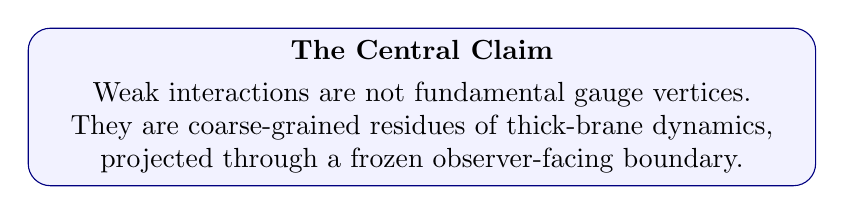
\begin{tikzpicture}
\node[rectangle, rounded corners=8pt, draw=blue!50!black, fill=blue!5,
      minimum width=10cm, minimum height=2cm, font=\normalsize, align=center]
{
\textbf{The Central Claim}\\[0.3em]
Weak interactions are not fundamental gauge vertices.\\
They are coarse-grained residues of thick-brane dynamics,\\
projected through a frozen observer-facing boundary.
};
\end{tikzpicture}
\end{center}

